\documentclass[12pt]{article}

%-------------PACKAGES------------- 
\usepackage[margin=1in]{geometry} 
\usepackage{amsmath,amsthm,amssymb}
\usepackage{pgfplots}
\usepackage{float}
\usepackage{braket}
\usepackage{titling}
\usepackage{tikz}
\usepackage{mathtools}
\usepackage{listings}
\usepackage{color}
\usepackage{caption}
\usepackage{subcaption}
\usepackage{algorithm,algpseudocode}

%-------------FORMATTING-------------
\setlength{\droptitle}{-6em} 
\setlength{\parindent}{0pt}
 
%--------------COMMANDS--------------
\newcommand{\N}{\mathbb{N}}
\newcommand{\Z}{\mathbb{Z}}
\newcommand{\R}{\mathbb{R}}
\newcommand{\C}{\mathbb{C}}
%\renewcommand{\qedsymbol}{\filledbox}

\DeclarePairedDelimiter \abs{\lvert}{\rvert}%
\DeclarePairedDelimiter \babs{\bigg\lvert}{\bigg\rvert}%
\DeclarePairedDelimiter \norm{\lVert}{\rVert}%

%------------ENVIRONMENTS------------- 
\newenvironment{theorem}[2][]{\begin{trivlist}
\item[{\bfseries #1}\hskip \labelsep {\bfseries #2.}]}{\end{trivlist}}
\newenvironment{lemma}[2][Lemma]{\begin{trivlist}
\item[\hskip \labelsep {\bfseries #1}\hskip \labelsep {\bfseries #2.}]}{\end{trivlist}}
\newenvironment{exercise}[2][Exercise]{\begin{trivlist}
\item[\hskip \labelsep {\bfseries #1}\hskip \labelsep {\bfseries #2.}]}{\end{trivlist}}
\newenvironment{reflection}[2][Reflection]{\begin{trivlist}
\item[\hskip \labelsep {\bfseries #1}\hskip \labelsep {\bfseries #2.}]}{\end{trivlist}}
\newenvironment{proposition}[2][Proposition]{\begin{trivlist}
\item[\hskip \labelsep {\bfseries #1}\hskip \labelsep {\bfseries #2.}]}{\end{trivlist}}
\newenvironment{corollary}[2][Corollary]{\begin{trivlist}
\item[\hskip \labelsep {\bfseries #1}\hskip \labelsep {\bfseries #2.}]}{\end{trivlist}}
\theoremstyle{remark}
\newtheorem*{remark}{Remark}

%-------------CODE-STYLE------------
\definecolor{dkgreen}{rgb}{0,0.6,0}
\definecolor{gray}{rgb}{0.5,0.5,0.5}
\definecolor{mauve}{rgb}{0.58,0,0.82}
\lstset{frame=tb,
	language=C++,
	aboveskip=3mm,
	belowskip=3mm,
	showstringspaces=false,
	columns=flexible,
	basicstyle={\small\ttfamily},
	numbers=none,
	numberstyle=\tiny\color{gray},
	keywordstyle=\color{blue},
	commentstyle=\color{dkgreen},
	stringstyle=\color{mauve},
	breaklines=true,
	breakatwhitespace=true,
	tabsize=3
}

\lstset{
	morekeywords={end}
}

%------------------------------------ 
%---------START-OF-DOCUMENT----------
%------------------------------------

\begin{document}
 
\title{Homework 8}
\author{David Miller \\ 
MAP5345: Partial Differential Equations I} 
 
\maketitle

\section*{Problem 1}

\textit{Consider the beam equation as in HW 7. Now suppose that the initial conditions are given by}
\begin{align}
	u_0(x) & = X_1 + \frac{1}{2}X_2 + \frac{1}{4}X_3 \\
	\dot{u}_0(x) & = 0
\end{align}
\textit{a) Write down the exact solution to the IBVP. Using Julia, plot the first three eigenfunctions, then plot a few different time values of the solution to visualize how a beam vibrates} \\

From the previous homework we have that the general solution to the PDE is 
\begin{align*}
		u(x,t) & = \sum\limits_{n=1}^\infty A_nT_n(t)X_n(x) \\
		T_n(t) & = u_0(x)cos(\sqrt{K\lambda_n}t) + \dot{u}_0(x)sin(\sqrt{K\lambda_n}t) \\
		X_n(x) & = \bigg(cosh(\sqrt[4]{\lambda_n}x) - cos(\sqrt[4]{\lambda_n}x)\bigg) - \frac{cosh(\sqrt[4]{\lambda L}) + cos(\sqrt[4]{\lambda L})}{sinh(\sqrt[4]{\lambda L}) + sin(\sqrt[4]{\lambda L})}\bigg(sinh(\sqrt[4]{\lambda_n}x) - sin(\sqrt[4]{\lambda_n}x)\bigg)
\end{align*}
From our initial conditions we can see that the $sin()$ component drops out and $A_1 = 1, A_2 = \frac{1}{2}$, and $A_3 = \frac{1}{4}$. Using Newton's method where the root we are computing is $cosh(\sqrt[4]{\lambda})cos(\sqrt[4]{\lambda}) + 1 = 0$ we get that $\lambda_3 \approx 3807, \lambda_2 \approx 485.5,$ and $\lambda_1 \approx 12.36$. From this we have 
\begin{align*}
	& u(x,t) = \\
	& \bigg[cosh(\sqrt[4]{\lambda_1}x) - cos(\sqrt[4]{\lambda_1}x) - \frac{cosh(\sqrt[4]{\lambda_1 L}) + cos(\sqrt[4]{\lambda_1 L})}{sinh(\sqrt[4]{\lambda_1 L}) + sin(\sqrt[4]{\lambda_1 L})}\bigg(sinh(\sqrt[4]{\lambda_1}x) - sin(\sqrt[4]{\lambda_1}x)\bigg)\bigg]cos(\sqrt{K\lambda_1}t) + \\
	& \frac{1}{2}\bigg[cosh(\sqrt[4]{\lambda_2}x) - cos(\sqrt[4]{\lambda_2}x) - \frac{cosh(\sqrt[4]{\lambda_2 L}) \, + cos(\sqrt[4]{\lambda_2 L})}{sinh(\sqrt[4]{\lambda_2 L}) + sin(\sqrt[4]{\lambda_2 L})}\bigg(sinh(\sqrt[4]{\lambda_2}x) - sin(\sqrt[4]{\lambda_2}x)\bigg)\bigg]cos(\sqrt{K\lambda_2}t) \, + \\
	& \frac{1}{4}\bigg[cosh(\sqrt[4]{\lambda_3}x) - cos(\sqrt[4]{\lambda_3}x) - \frac{cosh(\sqrt[4]{\lambda_3 L}) \, + cos(\sqrt[4]{\lambda_3 L})}{sinh(\sqrt[4]{\lambda_3 L}) + sin(\sqrt[4]{\lambda_3 L})}\bigg(sinh(\sqrt[4]{\lambda_3}x) - sin(\sqrt[4]{\lambda_3}x)\bigg)\bigg]cos(\sqrt{K\lambda_3}t)
\end{align*} \\

\begin{figure}[H]
	\centering
	\begin{subfigure}{.5\textwidth}
		\centering
		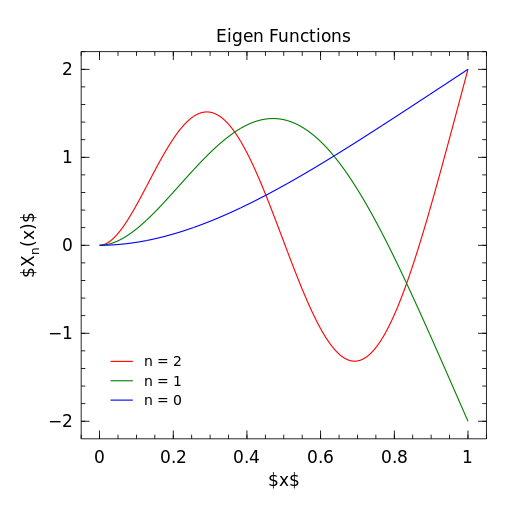
\includegraphics[width=1.025\linewidth]{Q1_EigenFunctions.png}
		\caption{Eigenfunctions $X_n$ of the PDE}
		\label{fig:sub1}
	\end{subfigure}%
	\begin{subfigure}{.5\textwidth}
		\centering
		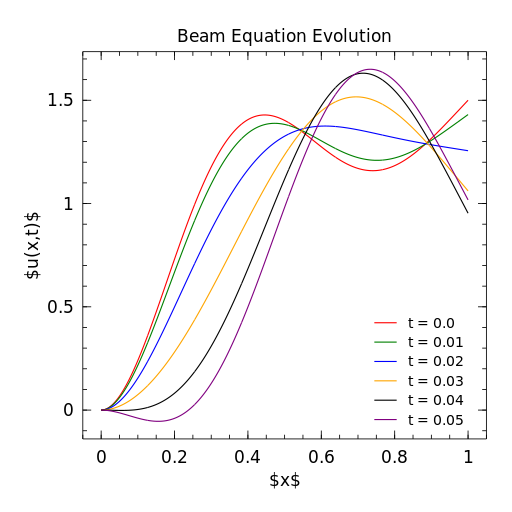
\includegraphics[width=1.025\linewidth]{Q1_BeamEq.png}
		\caption{Solution to Beam Equation with K = L = 1}
		\label{fig:sub2}
	\end{subfigure}
	\label{fig:test}
\end{figure}

\begin{figure}[H]
	\centering
	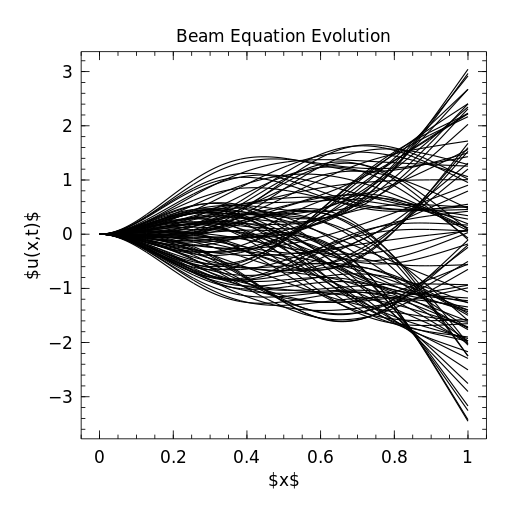
\includegraphics[width=10cm]{Q1_BeamEq_1.png}
	\caption*{Evolution of the beam for $t \in [0,1]$ with $dt = 0.01$}
\end{figure}

\newpage

\textit{b) Comparing your solution to the solution of the wave equation (for a plucked string), can you explain why a tuning fork has a 'purer' tone than a stringed instrument?} \\

\begin{figure}[H]
	\centering
	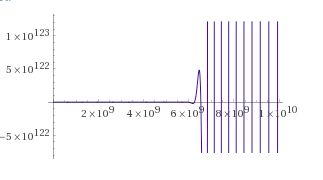
\includegraphics[width=10cm]{eigenvals.png}
	\caption*{Plot of $y = cos(\sqrt[4]{\lambda})cosh(\sqrt[4]{\lambda}) + 1$ for $\lambda \in [0,10^{10}]$}
\end{figure}


As we can see from the above graph the values of $\lambda$ become uniformly spaced. This leads to a constant frequency which is the "purer" tone the tuning fork gives over a plucked string. 

\newpage

\section*{Problem 2}

\textit{Consider the inner product for real-valued functions on the interval (-L,L)}
\begin{align}
	\braket{f,g} = \int\limits_{-L}^L f(x)g(x) \, dx
\end{align}
\textit{Prove that sin(n$\pi$x/L) and cos(m$\pi$x/L) are orthogonal for all non-negative integers n and m.} \\

Taking the inner product of $sin(n\pi x/L)$ and $cos(m\pi x/L)$ we get
\begin{align*}
	\braket{sin(\frac{n\pi x}{L}), cos(\frac{m\pi x}{L})} & = \int\limits_{-L}^L sin(\frac{n\pi x}{L})cos(\frac{m \pi x}{L}) \, dx \\
	& =
	\frac{1}{4i}\int\limits_{-L}^L (e^{in\pi x/L} - e^{-in\pi x/L})(e^{im\pi x/L} + e^{-im\pi x/L}) \, dx \\
	& = \frac{1}{4i}\int\limits_{-L}^{L}\bigg( e^{i(n+m)\pi x/L} + e^{i(n-m)\pi x/L} - e^{-i(n-m)\pi x/L} - e^{-i(n+m)\pi x/L} \, \bigg) dx \\
	& = \frac{1}{2}\int\limits_{-L}^L sin(\frac{(n+m)\pi x}{L}) + sin(\frac{(n-m)\pi x}{L}) \, dx = 0 \tag{$n \neq m$} \\
	\braket{sin(\frac{n\pi x}{L}), cos(\frac{n\pi x}{L})} & = 
	\int\limits_{-L}^L sin(\frac{n\pi x}{L})cos(\frac{n\pi x}{L}) \, dx \\ 
	& = -\frac{L}{2n\pi}cos^2(\frac{n\pi x}{L})\bigg\vert_{-L}^L = -\frac{L}{2n\pi}(cos(-n\pi) - cos(n\pi)) = 0 \tag{$n = m$}
\end{align*}
where we have used the fact that $\int_{-a}^a f(x) = 0$ for an odd function. Therefore we have that the functions $sin(n\pi x/L)$ and $cos(m\pi x/L)$ are orthogonal for all non-negative integers $n$ and $m$.

\newpage

\section*{Problem 3}

\textit{Let $f: [-\pi, \pi] \rightarrow \R$ be any function. Prove that if $f$ can be represented by a Fourier series, then the Fourier series is unique.} \\

Assume $f$ has two unique Fourier representations 
\begin{align*}
	f(x) = \sum\limits_{n = -\infty}^\infty c_n e^{inx}, \quad f(x) = \sum\limits_{n = -\infty}^\infty d_ne^{inx}
\end{align*}
where $c_n \neq d_n$ and for all $n$. Taking the difference of the two Fourier series we get
\begin{align*}
	f(x) - f(x) = 0 = \sum\limits_{n=-\infty}^\infty (c_n-d_n)e^{inx}
\end{align*}
To determine the coefficient $c_n - d_n$ we use projection
\begin{align*}
	c_n - d_n = \frac{\braket{0, X_m}}{\braket{X_n, X_m}} = 0
\end{align*}
where $X_n = e^{inx}$. Since $c_n - d_n = 0$ it follows that $c_n = d_n$ and therefore we have that $f$ has a unique Fourier representation.

\newpage

\section*{Problem 4}

\textit{Consider the functions $X_n = sin((n+1/2)\theta)$ over the interval $\theta \in [-\pi, \pi]$. Remember, to complete the proof of pointwise convergence of Fourier series, we need to fill a few gaps about $X_n$.} \\ \\
\textit{a) Prove that $\{X_n\}_{n=1}^\infty$ is an orthogonal set of functions.} \\

Taking the inner product of $X_n$ with itself we get
\begin{align*}
\braket{X_n, X_m} & = \int\limits_{-\pi}^\pi X_n(\theta)X_m(\theta) \, d\theta \\
& = \int\limits_{-\pi}^\pi sin((n+1/2)\theta)sin((m+1/2)\theta) \, d\theta \\
& = -\frac{1}{4}\int\limits_{-\pi}^{\pi} (e^{i(n+1/2)\theta} - e^{-i(n+1/2)\theta})(e^{i(m+1/2)\theta} - e^{-i(m+1/2)\theta}) \, d\theta \\
& = -\frac{1}{4}\int\limits_{-\pi}^{\pi} \bigg( e^{i(n+m+1)\theta} - e^{i(n-m)\theta} - e^{-i(n-m)\theta} + e^{-i(n+m+1)\theta} \bigg) \, d\theta \\
& = -\int\limits_{-\pi}^{\pi} cos((n+m+1)\theta) - cos((n-m)\theta) \, d\theta \\ 
& = \bigg( \frac{1}{n+m+1}sin((n+m+1)\theta) - \frac{1}{n-m}sin((n-m)\theta) \bigg)\bigg\vert_{\pi}^{-\pi} = 0 \tag{$n \neq m$} \\	
\end{align*}
Therefore we have shown that $\{X_n\}_{n=1}^\infty$ are an orthogonal set of functions. \\ 

\newpage

\textit{b) Calculate the $L^2$ norm for each $X_n$.} \\

We have that $\norm{X_n}_2 = \sqrt{\braket{X_n, X_n}}$, therefore we have
\begin{align*}
	\norm{X_n}_2 & = \bigg( \int\limits_{-\pi}^\pi X_n(\theta)X_n(\theta) \, d\theta \bigg) ^{1/2 }\\ 
	& = \bigg( \int\limits_{-\pi}^{\pi} sin^2((n+1/2)\theta) \, d\theta \bigg)^{1/2} \\
	& = \bigg( -\frac{1}{4}\int\limits_{-\pi}^{\pi} ( e^{i(n+1/2)\theta} - e^{-i(n+1/2)\theta} )^2 \, d\theta \bigg)^{1/2} \\ 
	& = \bigg( -\frac{1}{4}\int\limits_{-\pi}^{\pi} e^{2i(n+1/2)\theta} + e^{-2i(n+1/2)\theta} - 2 \,	 d\theta \bigg)^{1/2} \\ 
	& = \bigg( \pi - \frac{1}{2}\int\limits_{-\pi}^{\pi} cos((2n+1)\theta) \, d\theta \bigg)^{1/2} \\ 
	& = \bigg( \pi - \frac{1}{2n+1}sin((2n+1)\theta)\bigg\vert_{-\pi}^{\pi} \bigg)^{1/2} = \sqrt{\pi}
\end{align*}
We have shown that the $L^2$ norm for each $X_n$ is $\sqrt{\pi}$.
\newpage

\section*{Problem 5}

\textit{Using Julia, plot the Dirichlet kernel $K_n(\theta)$ = $sin((n+1/2)\theta)/sin(\theta/2)$ on the interval $\theta \in [-\pi, \pi]$ for a few different n values. What is the value of $K_n(\theta)$ at $\theta = 0$? Consider the convolution of a smooth function $f(x)$ against this kernel}
\begin{align}
	g(x) = \int\limits_{-\pi}^\pi K_n(\theta) f(x + \theta) \, d\theta
\end{align}
\textit{Give a loose argument for why this convolution picks out the value of f at x as $n \rightarrow \infty$.}

\begin{figure}[H]
	\centering
	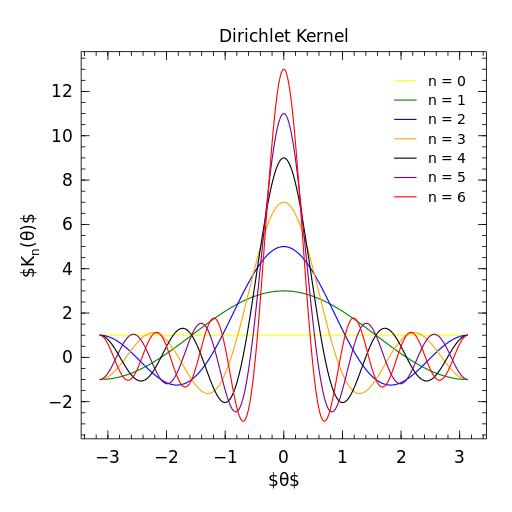
\includegraphics[width=10cm]{Q5.png}
\end{figure}
To find the value of $K_n(\theta)$ at $\theta = 0$ we simply take the limit
\begin{align*}
	\lim\limits_{\theta \rightarrow 0} K_n(\theta) = \lim\limits_{\theta \rightarrow 0} \frac{sin((n+1/2)\theta)}{sin(\theta/2)} = \lim\limits_{\theta \rightarrow 0} \frac{(n+1/2)cos((n+1/2)\theta)}{(1/2)cos(\theta/2)} = 2n+1
\end{align*}
Therefore we have that $K_n(0) = 2n+1$. The graph above agrees with our conclusion. 

\newpage

It is well known that for the Dirichlet Kernel $K_n(\theta)$ as $n \rightarrow \infty$ it converges to the Dirac Delta function $\delta(\theta)$. We can see this by plotting $K_n(\theta)$ for large $n$ values

\begin{figure}[H]
	\centering
	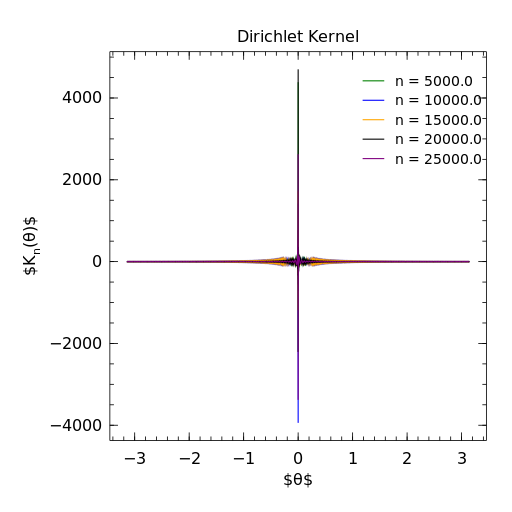
\includegraphics[width=10cm]{Q5_1.png}
\end{figure}

Using the fact that 
\begin{align*}
\int\limits_{-\infty}^\infty \delta(\theta - \theta^\star)f(x - \theta) \, d\theta = f(x)
\end{align*}
we get that the convolution of $f$ against the Dirichlet Kernel tends to $f(x)$ as $n \rightarrow \infty$, in this case we have that $\theta^\star = 0$.

\newpage

\section*{Problem 6}

\textit{Consider the piecewise function defined on the interval (-L,L)}
\begin{align}
	f(x) = 
	\begin{cases}
	1 & \text{if } 0 < x < L \\
	-1 & \text{if } -L < x < 0 \\
	0 & \text{if } x = 0
	\end{cases}
\end{align}
\textit{From the theorem we proved in class, we know that this function has a piecewise convergent Fourier series.} \\ \\
\textit{a) Using the complex form of the Fourier series, find each of the coefficients.} \\ 

The function $f(x)$ can be represented by a complex Fourier series via
\begin{align*}
	f(x) = \sum\limits_{n=-\infty}^\infty c_ne^{in\pi x/L}
\end{align*}
from which we can derive an expression for $c_n$ 
\begin{align*}
	\int\limits_{-L}^{L} f(x) e^{-im\pi x/L} \, dx  & = \int\limits_{-L}^{L} \bigg( \sum\limits_{n=-\infty}^\infty c_ne^{in\pi x/L} \bigg)e^{-im\pi x/L} \, dx \\
	& = \sum\limits_{n=-\infty}^\infty c_n \int\limits_{-L}^L e^{i(n-m)\pi x/L} \, dx \\
	& = \sum\limits_{n=-\infty}^\infty 2L c_n\delta_{nm} = 2L c_n \\
	\Rightarrow \quad c_n & = \frac{1}{2\pi}\int\limits_{-L}^L f(x)e^{-in\pi x/L} \, dx
\end{align*}
Therefore we can calculate the coefficients for $f(x)$'s complex Fourier series
\begin{align*}
	c_n & = \frac{1}{2L}\int\limits_{0}^{-L} e^{in\pi x/L} \, dx + \int\limits_0^L e^{in\pi x/L} \, dx \\
	& = \frac{i}{2n\pi}(e^{-in\pi} - 1 + e^{in\pi} - 1) \\
	& = -\frac{2i}{n\pi} \text{ when $n$ is odd}, 0 \text{ when $n$ is even}
\end{align*}

\newpage

\textit{b) Using this result, convert to a real Fourier series. Are there any symmetries in the problem that you can use as a sanity check on your result? What is the decay rate of the coefficients? Does your series converge absolutely?} \\

Using what we found in a previous homework we have that 
\begin{align*}
	a_n = 2\mathcal{R}(c_n), \quad b_n = 2\mathcal{I}(c_n) \, \text{ for } \, n \geq 1
\end{align*}
where $\mathcal{R}$ and $\mathcal{I}$ are the real and imaginary component, respectively. Thus the real Fourier series of $f$ is
\begin{align*}
	f(x) = \sum\limits_{n=1}^\infty \frac{4}{(2n-1)\pi}sin(\frac{(2n-1)\pi x}{L})
\end{align*}
where we can see that the decay rate is linear, that is $\frac{1}{n}$. We can do a sanity check by realizing the fact that an odd function times and odd function is even, an even function times an even function is even, and an odd function times an even function is odd. The other fact we use is that the integral of an odd function over a symmetric domain is zero. Therefore its easy to verify when we project to find $a_0$ we should get $a_0 = 0$. \\

Taking the absolute value of the series we get
\begin{align*}
\babs{ \frac{4}{(2n-1)\pi}sin(\frac{(2n-1)\pi x}{L})} & = \frac{4}{(2n-1)\pi}\babs{sin(\frac{(2n-1)\pi x}{L})} \\
& \geq \frac{4}{(2n-1)\pi}sin^2(\frac{(2n-1)\pi x}{L}) \\
& \geq -\frac{4}{(2n-1)\pi} \\
& \geq -\frac{4}{2\pi}\frac{1}{n} \\
& = -\frac{2}{\pi}\frac{1}{n}
\end{align*}
and thus does not converge absolutely by the $p$-series test.

\newpage

\section*{Problem 7}

\textit{Consider a function $f: [-\pi, \pi] \rightarrow \R$. If f(x) is an even function, prove that the Fourier series reduces to a cosine-series. If f(x) is odd, prove it is a sine-series.} \\

If $f(x)$ is even we have that $f(-x) = f(x)$. Translating this into $f(x)$'s Fourier series representation we have that 
\begin{align*}
	\underbrace{\frac{1}{2}a_0 + \sum\limits_{n=1}^\infty a_n cos(nx) + b_nsin(nx)}_{f(x)} = \underbrace{\frac{1}{2}a_0 + \sum\limits_{n=1}^\infty a_n cos(nx) - b_nsin(nx)}_{f(-x)}
\end{align*}
where we have used the fact that $sin(-\theta) = -sin(\theta)$ and $cos(-\theta) = cos(\theta)$. Subtracting $f(x)$ from both sides we are left with 
\begin{align*}
	\sum\limits_{n=1}^\infty 2b_nsin(nx) = 0
\end{align*} 
Using projection to determine the coefficient $b_n$ we get that 
\begin{align*}
b_n = \frac{1}{2}\frac{\braket{0, sin(mx)}}{\braket{sin(nx)}, sin(mx)} = 0	
\end{align*}
which implies an even function reduces to a cosine-series. Applying the same proof to an odd function, $f(-x) = -f(x)$, we start off with 
\begin{align*}
	\underbrace{-\frac{1}{2}a_0 - \sum\limits_{n=1}^\infty a_n cos(nx) + b_nsin(nx)}_{-f(x)} = \underbrace{\frac{1}{2}a_0 + \sum\limits_{n=1}^\infty a_n cos(nx) - b_nsin(nx)}_{f(-x)}
\end{align*}
where we have again used the fact that $sin(-\theta) = -sin(\theta)$ and $cos(-\theta) = cos(\theta)$. Now adding $f(x)$ to both sides we are left with
\begin{align*}
	\sum\limits_{n=0}^\infty 2a_ncos(nx) = 0 
\end{align*}
Using projection to determine the coefficient $a_n$ we get that 
\begin{align*}
a_n = \frac{1}{2}\frac{\braket{0, cos(mx)}}{\braket{cos(nx)}, cos(mx)} = 0	
\end{align*}
which implies an odd function reduces to a sine-series.

\end{document}